\documentclass{article}
\usepackage[utf8]{inputenc}

\usepackage{listings}
\usepackage[hyperfootnotes=false]{hyperref}
\usepackage{exercise}

\usepackage{verbatim}

\usepackage{algorithm}
\usepackage{algorithmicx}
\usepackage[noend]{algpseudocode}

\usepackage[toc,page]{appendix}

\usepackage[secthm,mdthm]{evan}


\usepackage{graphicx}

\usepackage{color}

\begin{comment} % for black and white printing; see below
\definecolor{myseagreen}{RGB}{88,197,191}
\definecolor{mysalmon}{RGB}{255,160,122}
\definecolor{myred}{RGB}{255,102,102}
\definecolor{mypurple}{RGB}{225,145,255}
\end{comment}
\definecolor{myblack}{RGB}{0,0,0}
\definecolor{mywhite}{RGB}{255,255,255}

% for black and white printing
\definecolor{myseagreen}{rgb}{1.0,1.0,1.0}
\definecolor{mysalmon}{rgb}{1.0,1.0,1.0}
\definecolor{myred}{rgb}{1.0,1.0,1.0}
\definecolor{mypurple}{rgb}{1.0,1.0,1.0}

\usepackage{tikz}

\usetikzlibrary{calc,shapes.multipart,chains,arrows,positioning}

\tikzstyle{vertex}=[draw,fill=myseagreen,circle,minimum size=24pt,inner sep=0pt]

\tikzstyle{splitvertex}=[draw,fill=myseagreen,circle split,minimum size=24pt]

\usetikzlibrary{
  shapes.multipart,
  matrix,
  positioning,
  shapes.callouts,
  shapes.arrows,
  shapes.geometric,
  decorations.shapes,
  shapes,
  fit,
  arrows,
  positioning,
  trees,
  mindmap,
  calc}

\tikzset{
    squarecross/.style={
        draw, rectangle,minimum size=18pt, fill=myseagreen,
        inner sep=0pt, text=black,
        path picture = {
            \draw[black]
            (path picture bounding box.north west) -- 
            (path picture bounding box.south east)
            (path picture bounding box.south west) -- 
            (path picture bounding box.north east);
        }
    }
}

\lstset{language=Java}
 
\definecolor{codegreen}{rgb}{0,0.6,0}
\definecolor{codegray}{rgb}{0.5,0.5,0.5}
\definecolor{codepurple}{rgb}{0.58,0,0.82}
% \definecolor{backcolour}{rgb}{0.95,0.95,0.92}
\definecolor{backcolour}{rgb}{1,1,1}

\lstnewenvironment{mylstlisting}[1][]%
  {\noindent\minipage{\linewidth}\medskip 
   \lstset{
    backgroundcolor=\color{backcolour},   
    commentstyle=\color{codegreen},
    keywordstyle=\color{magenta},
    numberstyle=\tiny\color{codegray},
    stringstyle=\color{codepurple},
    basicstyle=\footnotesize,
    breakatwhitespace=false,         
    breaklines=true,                 
    captionpos=t,                    
    keepspaces=true,                 
    numbers=left,                    
    numbersep=5pt,                  
    showspaces=false,                
    showstringspaces=false,
    showtabs=false,                  
    tabsize=4,
   basicstyle=\ttfamily\footnotesize,
   frame=single,#1}}
  {\endminipage}

\usepackage{footnote}
\makesavenoteenv{tabular}
\makesavenoteenv{table}

\renewcommand{\arraystretch}{1.5}


\title{Advanced Graph Theory}
\author{Daniel Wisdom}
\date{September 29th, 2017}

\begin{document}

\maketitle

\section{Minimum Spanning Tree}

Consider a connected, undirected graph. A \textit{spanning tree} is a subgraph that is a tree and contains every vertex in the original graph. A \textit{minimum spanning tree} (MST) is a spanning tree such that the sum of the edge weights of the tree is minimized. If we had a graph of cities and the distances between them, the minimum spanning tree would be the shortest set of roads to build that made every city reachable from every other city.  Finding the minimum spanning tree uses union-find, which was discussed earlier.  

\begin{center}
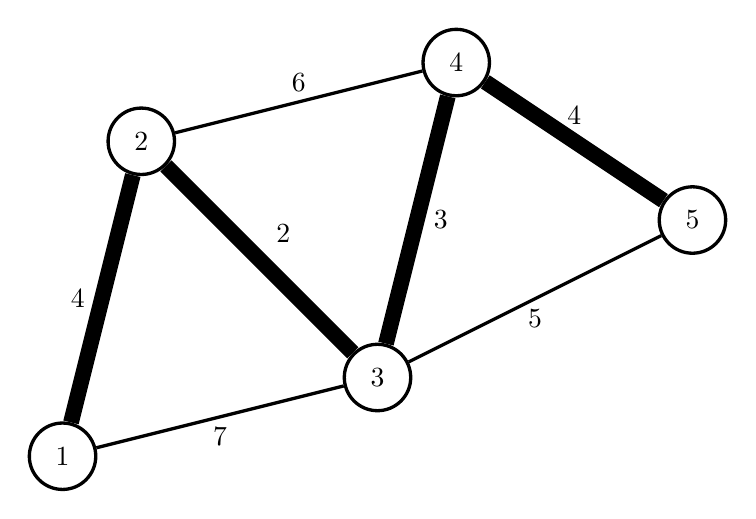
\begin{tikzpicture}[very thick,edge from parent/.style={draw,<-},level/.style={sibling distance=30mm/#1}]
\draw (0, 0) node [vertex] (v1) {1};
\draw (1, 4) node [vertex] (v2) {2};
\draw (4, 1) node [vertex] (v3) {3};
\draw (5, 5) node [vertex] (v4) {4};
\draw (8, 3) node [vertex] (v5) {5};
\draw[line width=2mm] (v1) -- (v2) node[midway, left] {4};
\draw[line width=2mm] (v2) -- (v3) node[midway, above right] {2};
\draw (v1) -- (v3) node[midway, below] {7};
\draw (v2) -- (v4) node[midway, above] {6};
\draw[line width=2mm] (v3) -- (v4) node[midway, right] {3};
\draw (v3) -- (v5) node[midway, below] {5};
\draw[line width=2mm] (v4) -- (v5) node[midway, above] {4};
\end{tikzpicture}
\end{center}


\subsection{Kruskal's Algorithm}

Kruskal's algorithm constructs an MST by greedily adding edges. We initialize every node as being in its own tree.  Then, loop over all edges in increasing order of weight.  If the edge connects two nodes in different trees, merge those trees and add that edge to the MST.  If an edge connects two vertices from the same tree, those two nodes are already connected and we just discard that edge. Conveniently, we have a union-find algorithm that can merge components and find the parent of  a node in basically linear time.

The MST of $n$ nodes always contains exactly $n-1$ edges, so we can stop looking through more edges after adding $n-1$ edges to the MST.

\begin{algorithm}[H]
\caption{Kruskal}
\begin{algorithmic}
\ForAll{edges $(u,v)$ in sorted order}
	\If{$\Call{Find}{u} \not= \Call{Find}{v}$}
		\State add $(u,v)$ to spanning tree
		\State $\Call{Union}{u,v}$
	\EndIf
\EndFor
\end{algorithmic}
\end{algorithm}


This algorithm requires a sort of the edges and thus has complexity $O(E \log{E}) = O(E \log{V})$.

\section{Shortest Paths}

\subsection{Floyd-Warshall}

Floyd-Warshall solves the shortest path problem for all pairs of vertices in $O(V^3)$ time, which is faster than $V$ single-source Dijkstra runs on a dense graph. Floyd-Warshall is very simple and quick to code, making it useful in contests with high execution time limits.  

The algorithm uses a table of the minimum distance between every pair of nodes.  Every entry in the table in initialized to $+\infty$.  The distance from each node to itself is 0.  The distance from the start to the end of each edge is also set to that edge's weight.

We then loop over every triple of nodes $k$, $i$, and $j$.  Node $k$ is the ``bridge" that connects pairs of $i$ and $j$.  Specifically, if $i$ can reach $k$ and $k$ can reach $j$, then the distance from $i$ to $j$ may be shortened to the sum of the distance from $i$ to $k$ and $k$ to $j$.  The order of these loops is important;  The ``bridge" node must always be the outermost loop.

Floyd-Warshall works on graphs with negative edge weights, unlike Dijkstra.  In graphs which contains cycles with net negative path weights the shortest path becomes $-\infty$.  Floyd Warshall will not report a length of $-\infty$, but it can easily be modified to detect negative cycles.  After the algorithm finishes we can check the distances from each node to itself.  If the $dist(i,i)<0$, node $i$ must be part of a negative cycle.



\begin{algorithm}[H]
\caption{Floyd-Warshall}
\begin{algorithmic}
\ForAll{vertices $v$}
	\State $dist(v,v)=0$
\EndFor
\ForAll{edges $(u,v)$}
	\State $dist(u,v)=weight(u,v)$
\EndFor
\ForAll{vertices $k$}
	\ForAll{vertices $i$}
    	\ForAll{vertices $j$}
        	\If{$dist(i,j) > dist(i,k)+dist(k,j)$}
            	\State $dist(i,j) \gets dist(i,k)+dist(k,j)$
            \EndIf
        \EndFor
    \EndFor
\EndFor
\end{algorithmic}
\end{algorithm}

\subsection{Bellman-Ford}

Bellman-Ford is a single-source $O(VE)$ shortest path algorithm that works when edge weights can be negative. It is preferable to Floyd-Warshall when the graph is sparse and we only need the answer for one source. Like Floyd-Warshall, the algorithm fails if the graph contains a negative cycle, but the algorithm is still useful for detecting negative cycles.

The key observation here is that the shortest path, assuming no negative cycles, has length at most $V-1$.  If we loop over all edges and consider if they form a new shortest path to their endpoint we can find all shortest paths of length 1.  If we repeat this loop $V-1$ times we discover all paths of length up to $V-1$.

To detect a negative cycle we simply run the loop one last time.  If any shorter paths are discovered, then the optimal path is longer than $V-1$ nodes.  The only way this is possible is if there is a negative cycle.


\begin{algorithm}[H]
\caption{Bellman-Ford}
\begin{algorithmic}
\ForAll{vertices $v$}
	\State $dist(v)\gets\infty$
    \State $prev(v)\gets -1$
\EndFor
\State $dist(src) \gets 0$
\For{$i=1$ to $V-1$}
	\ForAll{edges $(u,v)$}
		\If{$dist(u)+weight(u,v) < dist(v)$}
    	    \State $dist(v) \gets dist(u)+weight(u,v)$
	        \State $prev(v) \gets u$
        \EndIf
	\EndFor
\EndFor
\ForAll{edges $(u,v)$}
	\Comment{check for negative cycles}
	\If{$dist(u)+weight(u,v) < dist(v)$}
   	    \State{negative cycle detected}
	\EndIf
\EndFor
\end{algorithmic}
\end{algorithm}

\section {Problems}

1. Silver, February 2015 USACO Contest Problem 3, Superbull:

\noindent
Given $N\leq2000$ teams and the ``excitement" caused by a match between every pair of teams, find the most excitement possible in a tournament.  The loser is eliminated after every game, but you get to pick who loses.

\noindent
2. Give an algorithm for finding the spanning tree with the smallest product of edge weights, assuming all edge weights are positive.

\noindent
3. Bessie the cow is walking through some very corrupt cities in Zimbabwe. The cities are
connected by a set of roads, and each road has some bandit associated with it. Some bandits
are stronger than her, and will require a specific fee -$X_i$ for one safe passage. Other bandits
are weaker than Bessie, so she can force them to give her up to $X_i$ amount of money each
time she traverses the road. Please help her compute the maximum amount of money she
can obtain on her journey from Harare to Kwekwe.

\end{document}
